\documentclass[11pt]{article}
\usepackage[margin=4cm]{geometry}                % See geometry.pdf to learn the layout options. There are lots.
\geometry{letterpaper}                   % ... or a4paper or a5paper or ...
%\geometry{landscape}                % Activate for for rotated page geometry
%\usepackage[parfill]{parskip}    % Activate to begin paragraphs with an empty line rather than an indent
\usepackage{algorithm}
\usepackage[noend]{algpseudocode}
\usepackage{graphicx}
\usepackage{amssymb,amsfonts}
\usepackage{epstopdf}
\usepackage{multicol}
\usepackage{multirow}
\DeclareGraphicsRule{.tif}{png}{.png}{`convert #1 `dirname #1`/`basename #1 .tif`.png}
\setlength\parindent{8mm}
\title{Evacuating Priority Agents in a Disk with Unknown Exit Location}
\author{David Bushta, Christopher Till, Sunil Shende}
%\date{}                                           % Activate to display a given date or no date

\begin{document}
\maketitle
\section{Preliminaries}

\begin{flushleft}
Algorithms of search-and-escape involve mobile agents (also called Robots)
searching in geometric domains, such as a closed disk, or convex polygon. By
working together and communicating with one another, these mobile agents search
the domain to find an exit hidden on the perimeter. Many different problems have
previously been studied in this topic, such as finding algorithms to evacuate all
agents in a domain, or only evacuating a specific subset of these agents.
\end{flushleft}

\subsection{Model}

\begin{flushleft}

All agents in this problem use the same coordinate system and operate in a closed
disk, all starting from the center. These agents' algorithms do not all have to be the same,
and in fact to most efficiently search the circle, they must all be unique.
In our problem, we observe the Priority model of algorithms. In this model, a
subset of one or more agents (P) are defined as a Priority (or Queen) and the goal
of the algorithm is to evacuate a required subset of these Priority Agents. These
algorithms also include a number Helper agents (H), that simply assist in searching the circle
for the exit, for a total of (H + P) agents. The Helper agents are not required to evacuate.


\vspace*{5mm} \hspace{\parindent} Once an exit is found, whether by a Helper or a Priority, the agent may use
Wireless communication to immediately broadcast the exit's location and its own identity to all other agents.
Upon receiving this broadcasted location, any remaining Priority agents that
need to evacuate travel along a chord to the exit and when the required subset has exited, the algorithm terminates.
The cost of the algorithm is called the termination time, and is the total worst-case
time for the required subset of Priority agents to exit.
\end{flushleft}

\subsection{Previous Work}

\begin{flushleft}
Similar search-and-evacuate problems to this one have previously been studied, including those involving Agents
searching on a line, and searching inside of other types of shapes, such as a triangle.
In our research thus far, we have mainly looked at the problems regarding
the closed unit disk and how to most efficiently search for the exit and evacuate
different subsets of agents. We started by studying the algorithms that have been designed
for $n = 2, 3$ agents using both the face-to-face and wireless communication models [(Evacuating Robots
From a Disk Using Face-to-Face Communication, 2015), (Evacuating Robots Via an Unknown Exit in a Disk, 2015)].
In these algorithms, all agents must evacuate for the algorithm to terminate, and there is no notion of
Priority of Helper. Interestingly, in the face-to-face model, agents must be next to each other to
communicate.

\vspace*{5mm} \hspace{\parindent} Afterwards, we looked at problems of a similar type that have been studied,
namely those regarding 1 Priority and 1 or more Helper agents searching in a
closed disk solely usign wireless communication (God Save the Queen, 2018)
(Priority Evacuation From a Disk Using Mobile Robots, 2018)].
In these papers, the results involved getting the only Priority agent to the exit
as fast as possible, however, our problem attempts to design an algorithm where
only one of multiple Priority agents needs to evacuate.

\vspace*{5mm} \hspace{\parindent} To facilitate studying these algorithms and seeing results based on test data, we
have created an algorithm visualizer. This program uses the different types of movement and
communication directives we commonly see in each algorithm to recreate an
interactive visualization of the algorithm. To date, all of the algorithms
listed in the above papers including our own can be shown, and new ones can be created.
\end{flushleft}


\subsection{Our Results}

\begin{flushleft}
\hspace{\parindent} In our algorithm using 2 Priority and 1 Helper agent with 1 Priority required to exit, we show that a termination time
upper bound of \textbf{3.55 time units} is possible given the specific set of parameters we use
to guide the agents. We can achieve this by using a \textbf{parameter of angle $\alpha = 5 \pi / 9 - 2\sqrt3 /3$} for the two agents to travel to the perimeter in the third quadrant, i.e, they travel out at
an angle of \textbf{$\pi + \alpha$}. This allows us to set the two worst-case time predictions equal.
These are the cases where \textbf{$A)$} $P2$ finds the exit at the very end of its search,
or \textbf{$B)$} $H$ finds the exit in the second quadrant at the angle \textbf{$\pi - \beta$},
where \textbf{$\beta = ( \pi / 3 - \alpha) / 2$}.
\end{flushleft}




\section{Upper Bound}

\subsection {Evacuation Algorithm for 2 Priority \& 1 Helper}

%Our first priority algorithm with 2 queens and 1 servant
\begin{center}
    \begin{tabular}{ | p{1.5cm} || r l | }
        \hline
        \multicolumn{3} { | c | }{ Algorithm \textbf{2 Priority 1 Helper}($\alpha$)} \\ \hline
        \textbf{Robot} & $\textbf{\#}$ & \textbf{Trajectory} \\  \hline
        \multirow{2}{*}{$P1$} & 0 & Travel from $O$ to $C_{0}$ \\
        & 1 & Travel CCW until exit is found. \\  \hline
        \multirow{2}{*}{$P2$} & 0 & Travel from $O$ to $C_{\pi + \alpha}$ \\
        & 1 & Travel CCW until exit is found.\\ \hline
        \multirow{4}{*}{$H$} & 0 & Travel from $O$ to $C_{\pi + \alpha}$ \\
        & 1 & Travel CW until exit is found.\\
        & (2) & IF exit is found by $H$, broadcast location and wait.\\
        & (2) & ELSE Wait.\\ \hline
    \end{tabular}
\includegraphics{mypics/2Q1S_references.pdf} \hfill
\end{center}

\begin{center}
    \textbf{Figure 1}: Reference points.
\end{center}

\begin{flushleft}

\vspace*{5mm} \textbf{Lemma 1}: The upper bound of the distance between two speed-1 agents converging on an unexplored arc
of a unit disk with angle $a >= 2\pi/3$ occurs when the agents are $\sqrt{3}$ away from
each other at the time of exit discovery.
\begin{center}
    \includegraphics{mypics/lemma1-references.pdf}
\end{center}
\vspace*{5mm} \textbf{Proof}: Suppose the helper $H$ finds the exit at some point $B$ after the agents
have traveled a distance of $c$ along the arc. Then, the total time taken by the priority agent P
to get to $B$, having started at the opposite side of the arc $a$, would be:

\[ t = c + 2 \sin (\frac{a - 2c}{2}) \]

\vspace*{5mm} Then, differentiating with respect to $t$, we get:

\[ \frac{dt}{dc} = 1 - 2 \cos (\frac{a - 2c}{2}) \]

\vspace*{5mm} Finally, setting that equal to zero results in:

\[ \frac{2\pi}{3} = a - 2c \]

\vspace*{5mm} Thus, the greatest value for $t$ will occur when the agents are $\sqrt{3}$ apart,
or at an angle of $ \frac{2\pi}{3}$ for $a >= \frac{2\pi}{3}$.



\end{flushleft}

\subsection {Equations}

\begin{flushleft}
    First, we know that we can divide the circle into two sections, where $a$ is the
    responsibility of the Helper and Priority 1, and the $b$ is the responsibility of Priority 2.
    Therefore:

    \[ 2\pi = a + b \]

    We know that Priority 1 and Helper will have to travel a total of $a$ around the circle,
    and after a certain time $c$, the remaining unsearched area will be $d = a - 2c$, so at this point:

    \[ 2\pi = b + 2c + d \]

    If, after more time $e$ of both agents following the perimeter the distance between the two
    would be equal to $\sqrt{3}$, which by Lemma 1 will result in the evacuation time increasing, then
    we instead send Priority 1 along a chord of angle $h$, such that when Helper reaches point $C_{a - c - e}$, Priority 1 will be travelling somewhere along the chord. The point at which Priority 1 reaches the
    end of the detour at point $C_{c + h}$, the Helper will be at point $C_{a - c - e - f}$, where $f$ is the extra time taken by Priority 1 to reach the end of its detour.

    \[ e + f = 2\sin(\frac{h}{2}) \]

    We call $g$ the remaining unsearched arc between $C_{c + h}$ and $C_{a - c - e - f}$.
    At this point in the algorithm, we send Priority 1 clockwise to search the area from $C_{c + h}$ until
    $C_{c}$ and Helper stays clockwise to search the remaining area from $C_{a - c - e - f}$ until $C_{c + h}$. At this point the distance between the two agents stays constant for the rest of the algorithm, and this distance is equal to $2\sin(\frac{g}{2})$. Clearly, the optimal value for $h$ is:

    \[ h = g + 2\sin(\frac{g}{2})\]

    At this point, we have fully partitioned the circle such that:

    \[ 2\pi = b + 2c + e + f + g + h\]

    which, once simplified, becomes:

    \[ 2\pi = b + 2c + 2\sin(\frac{g + 2\sin(\frac{g}{2})}{2}) + 2g + 2\sin({g}{2}) \]

    At this point, we identify two upper bounds. One is when Priority 2 finds the exit at the end of its
    search, after time $t = 1 + b$, and the other is when either Helper or Priority 1
    finds the exit at the end of their search, after time $t = 1 + c + e + f + h$.

    \[b = c + e + f + h\]

     


\end{flushleft}

% \includegraphics{mypics/2Q1S_Initial.pdf}
% 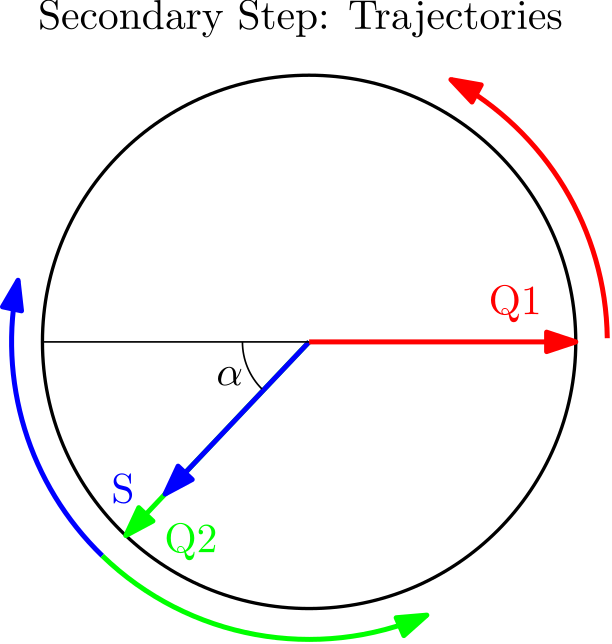
\includegraphics{mypics/2Q1S_Second_Step.pdf}
% \includegraphics{mypics/2Q1S_Initial.pdf}
% \includegraphics{mypics/2Q1S_Initial.pdf}

\end{document}
